\section{Experiments}
\label{sec:experiments}
In this section, we first describe our dataset, followed by our experimental setup; comparative baselines, evaluation metrics, and implementation details. We then present results across several experiments to evaluate the performance of our model on merging semantically diverse induced-relations. %We finally provide a brief analysis of our proposed contrastive modification to convolution, gradient boosting and their implications on model fitting.
%We then report the results of our boosted model and its variants. Furthermore, we evaluate against common aggregator approaches and finally study the robustness of our model to training label sparsity.
\begin{table*}[h]
 \centering
 \small
 \centering
  \setlength{\tabcolsep}{0.5pt}
   \begin{tabular}{l|c@{\hspace{0.3mm}}c@{\hspace{0.3mm}}c@{\hspace{0.3mm}}|c@{\hspace{1.0mm}}c@{\hspace{1.0mm}} c@{\hspace{1.0mm}} |c@{\hspace{1.0mm}}c@{\hspace{0.6mm}}c@{\hspace{0.5mm}}|c@{\hspace{0.8mm}} c@{\hspace{0.8mm}}c@{\hspace{0.8mm}}|c@{\hspace{0.3mm}}c@{\hspace{0.3mm}}c@{\hspace{0.3mm}} }
 %\begin{tabular}{l|c@{\hspace{0.8mm}}c@{\hspace{0.8mm}}c@{\hspace{0.8mm}}|c@{\hspace{1.2mm}}c@{\hspace{1.2mm}} c@{\hspace{1.2mm}} |c@{\hspace{1mm}}c@{\hspace{1mm}}c@{\hspace{1mm}}|c@{\hspace{1mm}} c@{\hspace{1mm}}c@{\hspace{1mm}}|c@{\hspace{1mm}}c@{\hspace{1mm}}c@{\hspace{1mm}} }
   %\begin{tabular}{l | r r r | r r r | c c c | r r r | r r r }
  % \resizebox{\columnwidth}{!}{%
  % \begin{tabular}{l*{4}S[tight-spacing=true]}
  \toprule
  &  \multicolumn{3}{c}{\textbf{Technology}} &
  \multicolumn{3}{c}{\textbf{Culture/Recreation}} &
  \multicolumn{3}{c}{\textbf{Life/Arts}} &
  \multicolumn{3}{c}{\textbf{Science}} &
  \multicolumn{3}{c}{\textbf{Professional/Business}}\\
  & ServerFault & AskUbuntu & Unix & English & Games & Travel & SciFi & Home & Academia & Physics & Maths & Statistics & Workplace & Aviation & Writing \\ \midrule
$\vert Q \vert$ & 61,873 & 41,192 & 9,207 & 30,616 & 12,946 & 6,782 & 14,974 & 8,022 & 6,442 & 23,932 & 18,464 & 13,773 & 8,118 & 4,663 & 2,932 \\
$\vert  \mathcal{A} \vert$ & 181,974 & 119,248 & 33,980 & 110,235 & 45,243 & 20,766 & 49,651& 23,956 & 23,837 & 65,800 & 53,772 & 36,022 & 33,220 & 14,137 & 12,009 \\
$ \vert U \vert$ & 140,676 & 200,208 & 84,026 & 74,592 & 14,038 & 23,304 & 33,754 & 30,698 & 19,088 & 52,505 & 28,181 & 54,581& 19,713 & 7,519 & 6,918 \\
$ \mu (\vert  \mathcal{A}_q \vert) $ & 2.94 & 2.89 & 3.69 & 3.6 & 3.49 & 3.06 & 3.31 & 2.99 & 3.7 & 2.75 & 2.91 & 2.62 & 4.09 & 3.03 & 4.10 \\
   \bottomrule
 \end{tabular}
 \caption{ \small \label{tab:stats}Dataset statistics for the top three Stack Exchange communities from five different categories. $\vert Q \vert$: number of questions; $\vert  \mathcal{A} \vert$: number of answers; $ \vert U \vert $: number of users; $ \mu (\vert  \mathcal{A}_q \vert) $: mean number of answers per question. Professional/Business communities have slightly more answers per question on average than others. Technology communities are the largest in terms of number of question out of the five categories.}
 \vspace{-0.2in}
\end{table*}

\subsection{Dataset}
%catering to topics ranging from open-ended discussions to fact-based questions
We evaluate our approach on multiple communities catering to different topics from a popular online Community Question Answer (CQA) platform, \emph{StackExchange\footnote{https://stackexchange.com/}}. The platform divides the communities into five different categories, i.e. Technology ($\mathbf{T}$), Culture/Recreation ($\mathbf{C}$), Life/Arts ($\mathbf{L}$), Science ($\mathbf{S}$) and Professional ($\mathbf{P}$).
For our analysis, we collect data from the ten largest communities from each of the five categories until March 2019, resulting in a total of 50 StackExchange communities. In StackExchange, each questioner can mark a candidate answer as an "accepted" answer. We only consider questions with an accepted answer. Table \ref{tab:stats} shows the final dataset statistics.

For each $(q, a)$ tuple, we compute the following basic features:\\
\emph{Activity features :} View count of the question, number of comments for both question and answer, the difference between posting time of question and answer, arrival rank of answer (we assign rank 1 to the first posted answer) \cite{TianZL13}. \\
\emph{Text features :} Paragraph and word count of question and answer body and question title, presence of code snippet in question and answer (useful for programming based forums)\\
\emph{User features :} Word count in user profile's Aboutme section for both users; one posting the question and other posting the answer.

Time-dependent features like upvotes/downvotes of the answer and user features like reputation or badges used in earlier studies on StackExchange \cite{BurelMA16} are problematic for two reasons. First, we only know the aggregate values, not how these values change with time. Second, since these values typically increase over time, it is unclear if an accepted answer received the votes \emph{prior} to or \emph{after} an answer was accepted. Thus, we do not use such time-dependent features for our model and the baselines in our experiments.


\subsection{Experimental Setup}
\subsubsection{Baselines} We compare against state-of-the-art feature-based baselines for answer selection and competing aggregation approaches to fuse diverse relational views of the dataset~\cite{DualGCN,relationalGCN}.

\noindent
\textbf{Random Forest (RF)} \cite{BurelMA16,TianZL13} model trains on the feature set mentioned earlier for each dataset. This model is shown to be the most effective feature-based model for Answer Selection.

\noindent
\textbf{Feed-Forward network (FF)} \cite{JendersKN16} is used as a deep learning baseline to learn non-linear transformations of the feature vectors for each $(q, a)$ tuple. This model is equivalent to our Reflexive GCN model in isolation.

\noindent
\textbf{Dual GCN (DGCN)} \cite{DualGCN} trains a separate GCN for each view. In addition to the supervised loss computed using training labels, they introduce a regularizer to minimize mean squared error (MSE) between vertex representations of two views, thus aligning the learned latent spaces.
%Formally,
%For instance,
%\begin{equation*}
%  \mathcal L_{reg}(Z_c, Z_{ts}) = \frac{1}{n} \sum_{j \in {1,n}}  \lVert Z_c^j - Z_{ts}^j \lVert
%\end{equation*}
%computes the MSE loss between Contrastive and TrueSkill Similarity GCN.
%\cite{DualGCN} proposed the model for two GCN representations.
%We extend the original two GCN model \cite{DualGCN} to four GCN, each representing our relational views between the nodes. We minimize the supervised loss with respect to the best performing GCN model (Contrastive), and its node representation's alignment with respect to all other GCN's node representations.
%The Contrastive view is seen to exhibit the best performance in isolation. Thus, the DualGCN loss can be given by:
%   \vspace{-0.09in}
% \begin{equation*}
%   %\mathcal L  = \mathcal L_0(Z_c) + \lambda{(t)} \left( \mathcal L_{reg}(Z_c, Z_{ts}) + \mathcal L_{reg}(Z_c, Z_{as}) + \mathcal L_{reg}(Z_c, Z_r) \right)
%   \mathcal L  = \mathcal L_0 +  \lambda{(t)} \left( \sum_{S_i \in \mathbf{S}, S_i \neq c} \lVert \mathbf{Z}_c^K - \mathbf{Z}_i^K \lVert \right)
% \end{equation*}
% where $\mathcal L_0$ represents the supervised loss and $\mathbf{Z}_c^K$ is the node representations of the Contrastive GCN.
The regularizer loss is similar to our intra-relation aggregation approach but assumes label and feature sharing across \emph{all} the views.

\noindent
\textbf{Relational GCN (RGCN)} \cite{relationalGCN} combines the output representations of previous layer of each view to compute an aggregated input to the current layer.
%$\mathbf{Z}_i^{k-1}$ of layer $k-1$ of each view to compute an aggregated input to layer $k$.
% Formally,
%
% \begin{equation*}
%   \mathbf{Z}_{rgcn}^{k} = \sigma \left( \sum_{S_i \in \mathbf{S}} \mathbf{Z}_i^{k-1}\right)
% \end{equation*}
% where $Z_{rgcn}$ is final output of this model at layer $k$ and $\sigma$ is the activation function.

We also report results for each view individually: Contrastive (C-GCN), Arrival Similarity (AS-GCN), TrueSkill Similarity (TS-GCN), and Reflexive (R-GCN) with our proposed IR-GCN model. We do not compare with other structure-based approaches to compute vertex representations \cite{DeepWalk,node2vec,LINE} as GCN is shown to outperform them \cite{gcn}. We also compare with common aggregation strategies to merge neural representations discussed earlier in ~\cref{sec:aggregation} later.
% in \cref{sec:agg}.

\subsubsection{Evaluation Metric}
%We divide the $(q, a)$ tuples into train and test set such that there is no overlap between the set of questions in the two set.
We randomly select 20\% of the questions, $\mathbf{T}_q \subset \mathcal{Q}$ to be in the test set. Then, subsequently all $(q,a)$ tuples such that $q \in \mathbf{T}_q$ comprise the set of test tuples or vertices, $\mathbf{T}$ . The rest of the vertices, along with their label information, is used for training the model.
%Note that each view, $G_i = (V, E_i)$ is defined over all nodes or tuples, $V$, in the data but the loss is only computed over the training set.
We evaluate our model on two metrics, Accuracy and Mean Reciprocal Rank (MRR). Accuracy metric is widely used in vertex classification literature while MRR is popular for ranking problems like answer selection. Formally,
\begin{align*}
%Acc = \frac{1}{\vert \mathcal{T} \vert \in T} \sum \mathbbm{1} (\mathop{\mathrm{sign}} \left( \mathbf{Y} \odot \mathbf{h}_b \right) > 0)
Acc = \frac{1}{\vert \mathbf{T} \vert} \sum_{(q,a) \in  \mathbf{T} } \mathbbm{1} \left(  y_{(q,a)} \cdot h_b((q,a)) > 0 \right)
\end{align*}
with $\cdot$ as the product and $\mathbbm{1}$ as the indicator function. The product is positive if the accepted label and predicted label match and negative otherwise.
\begin{equation*}
%MRR = \sum_{q \in Q} \left({R_{(q,a)}}^{-1} \right) \forall a \in A(q) \; \text{and} \; y_{(q,a)} = 1
MRR = \frac{1}{\vert \mathbf{T}_q \vert} \sum_{q \in \mathbf{T}_q} \frac{1}{\sum_{a' \in \mathcal{A}(q)}  \mathbbm{1} \left(L_{(q,a)} < L_{(q,a')} \right)} %\Bigg\vert \texttt{  }y_{(q,a)} = 1} %\right\rbrace
\end{equation*}
%\begin{align*}
%  Acc &= \frac{1}{n} \sum\limits_{i=1}^n \mathbbm{1} \left( y_i, h_b(x_i) \right)\\
%    MRR &= \sum\limits_{q=1}^{Q} \left(\frac{1}{R_a} \right) \forall a \in A(q) \; \text{and} \; y_a = 1
%\end{align*}
 where
%$\mathbf{T}_q$ is the set of questions in the test set and
$L_{(q,a)}$ is the position of accepted answer $a$ in the ranked list for question $q$ \cite{Wang:2009}.
 %MRR measure considers the position of the accepted answer in the ranked list. %Note that MRR is computed for each question in the test set while Accuracy is computed for all the $(q,a)$ tuples.

 \begin{table*}[h]
   %\robustify\bfseries
   %\small
   \centering
     \setlength{\tabcolsep}{0.5pt}
   \begin{threeparttable}
  %\begin{tabular}{l|S[round-mode=places,round-precision=2]@{\hspace{1mm}}S@{\hspace{1mm}}|S[round-mode=places,round-precision=2]@{\hspace{1mm}}S@{\hspace{1mm}}|S[round-mode=places,round-precision=2]@{\hspace{1mm}}S@{\hspace{1mm}}|S[round-mode=places,round-precision=2]@{\hspace{1mm}}S@{\hspace{1mm}}|S[round-mode=places,round-precision=2]@{\hspace{1mm}}S@{\hspace{1mm}}S[round-mode=places,round-precision=2]@{\hspace{1mm}}S@{\hspace{1mm}}}
  %\begin{tabular}{l|S[round-mode=places,round-precision=2]S|S[round-mode=places,round-precision=2]S|S[round-mode=places,round-precision=2]S|S[round-mode=places,round-precision=2]S|S[round-mode=places,round-precision=2]SS[round-mode=places,round-precision=2]S}
  %\resizebox{1.5\columnwidth}{!}{
  \begin{tabular}{l|c c|c c|c c|c c|c c}
     \toprule
     \multirow{2}{*}{Method} &
        \multicolumn{2}{c}{\textbf{Technology}} &
       \multicolumn{2}{c}{\textbf{Culture/Recreation}} &
       \multicolumn{2}{c}{\textbf{Life/Arts}} &
       \multicolumn{2}{c}{\textbf{Science}} &
       \multicolumn{2}{c}{\textbf{Professional/Business}}\\
       &{Acc(\%)} & {MRR}&{Acc(\%)} & {MRR}&{Acc(\%)}& {MRR}&{Acc(\%)} & {MRR}&{Acc(\%)} & {MRR}\\
       %\cmidrule(lr){1-1}\cmidrule(lr){2-21}%\cmidrule(lr){12-21}
       \midrule
     \textbf{RF~\cite{BurelMA16,TianZL13}} & 66.78$\pm$0.023 & 0.683$\pm$0.043 & 72.50$\pm$0.018 & 0.626$\pm$0.050 & 72.71$\pm$0.049 & 0.628$\pm$0.089 & 68.09$\pm$0.024 & 0.692$\pm$0.049 & 74.72$\pm$0.044 & 0.595$\pm$0.081\\


     \textbf{FF~\cite{JendersKN16}} & 67.31$\pm$0.027 & 0.786$\pm$0.022 & 72.22$\pm$0.020 & 0.782$\pm$0.023\textbf{*} & 73.58$\pm$0.049 & 0.780$\pm$0.034 & 67.87$\pm$0.024 & 0.800$\pm$0.028 & 74.63$\pm$0.040 & 0.760$\pm$0.049\\
     %biLSTM & 63.84 & 0.6887 & 64.40 & 0.6772 & 70.65 & 0.5679 & 58.27 & 0.6944 & 58.10 & 0.6939 & 64.31 & 0.5869 \\
     %biLSTM+CNN & 67.86 & 0.7115 & 68.95 & 0.7009 & 73.08 & 0.6253 & 61.15 & 0.7050 & 59.15 & 0.7279 & 66.75 & 0.5997 \\
     \textbf{DGCN~\cite{DualGCN}} & 70.70$\pm$0.022 & 0.782$\pm$0.017 & 75.22$\pm$0.017 & 0.772$\pm$0.028 & 76.73$\pm$0.034 & 0.784$\pm$0.038 & 71.45$\pm$0.023\textbf{*} & 0.792$\pm$0.035 & 76.86$\pm$0.031 & 0.751$\pm$0.046 \\
     \textbf{RGCN~\cite{relationalGCN}} & 54.40$\pm$0.045 & 0.673$\pm$0.045 & 60.39$\pm$0.016 & 0.646$\pm$0.042 & 59.97$\pm$0.043 & 0.655$\pm$0.054 & 58.65$\pm$0.054 & 0.683$\pm$0.042 & 63.02$\pm$0.038 & 0.657$\pm$0.061\\
     \cmidrule(lr){1-1}\cmidrule(lr){2-11}%\cmidrule(lr){12-21}
     \textbf{AS-GCN} & 67.76$\pm$0.032 &0.775$\pm$0.015 & 73.05$\pm$0.021 & 0.763$\pm$0.025 &73.79$\pm$0.048 & 0.777$\pm$0.042 & 66.93$\pm$0.045 & 0.788$\pm$0.028 & 74.99$\pm$0.045 & 0.742$\pm$0.047 \\
     \textbf{TS-GCN} & 66.87$\pm$0.032 & 0.779$\pm$0.018 & 72.16$\pm$0.023 & 0.764$\pm$0.023 & 72.02$\pm$0.061 & 0.766$\pm$0.048 & 65.90$\pm$0.042 & 0.790$\pm$0.031 & 74.17$\pm$0.046 &0.747$\pm$0.044\\
     \textbf{C-GCN } & 71.64$\pm$0.022\textbf{*} & 0.790$\pm$0.015\textbf{*}& 76.18$\pm$0.017\textbf{*}& 0.781$\pm$0.024 & 77.37$\pm$0.034\textbf{*}& 0.788$\pm$0.040\textbf{*} & 70.81$\pm$0.042 & 0.800$\pm$0.032\textbf{*}& 77.57$\pm$0.038\textbf{*} & 0.768$\pm$0.034\textbf{*} \\
     %\textbf{IR-GCN} & \bfseries 73.96 $\pm$ \bfseries 0.023 & \bfseries0.7939\ \ \  $\pm$ \bfseries 0.014 & \bfseries 78.61 $\pm$ \bfseries 0.018 & \bfseries 0.7905 \ \ \ $\pm$ \bfseries 0.025 & \bfseries 79.21 $\pm$ \bfseries 0.032 & \bfseries 0.7995 \ \ \ $\pm$ \bfseries 0.037 & \bfseries 74.98 $\pm$ \bfseries 0.021 & \bfseries 0.8085 \ \ \ $\pm$ \bfseries0.028 & \bfseries80.17 $\pm$ \bfseries 0.026 & \bfseries 0.7849 \ \ \ $\pm$ \bfseries 0.032\\
     \textbf{IR-GCN} & \textbf{73.96$\pm$0.023} & \textbf{0.794$\pm$0.014} & \bfseries 78.61$\pm$\bfseries0.018 & \bfseries 0.791$\pm$\bfseries 0.025 & \bfseries 79.21$\pm$\bfseries 0.032 & \bfseries 0.800$\pm$\bfseries 0.037 & \textbf{74.98$\pm$0.021} & \textbf{0.809$\pm$0.028} & \textbf{80.17$\pm$0.026} & \textbf{0.785$\pm$0.032} \\
     \bottomrule
   \end{tabular}
   %}
   \begin{tablenotes}
       \footnotesize
       \item[*] DGCN stands for DualGCN, RGCN stands for RelationalGCN, and IR-GCN stands for Induced Relational GCN.
   \end{tablenotes}
   \caption{\small \label{tab:stackacc} Accuracy and MRR values for StackExchange with state-of-the-art baselines. Our model outperforms by at least 4\% in Accuracy and 2.5\% in MRR. Contrastive GCN performs best among individual views. The model with $*$ symbol has the second-best performance among all other models. Our model shows statistical significance at level 0.01 overall second best model on single tail paired t-test.}
   \end{threeparttable}
 \vspace{-0.2in}
 \end{table*}

\subsubsection{Implementation Details}
We implemented our model and the baselines in Pytorch. We use ADAM optimizer \cite{ADAM} for training with 50\% dropout to avoid overfitting. We use four hidden layers in each GCN with hidden dimensions 50, 10, 10, 5, respectively, and ReLU activation. The coefficients of $\mathcal{L}_1$ and $\mathcal{L}_2$ regularizers are set to $\gamma_1 = 0.05$ and $\gamma_2 = 0.01$ respectively. For TrueSkill Similarity, we use margin $\delta = 4$ to create links, while for Arrival similarity, we use $\delta = 0.95$.
%The weight decay for annealing schedule $\lambda(t)$ is set to $\exp^{-t/20}$.
We implement a mini-batch training for large graphs where each batch contains a set of questions and their associated answers. This is equivalent to training on the whole graph as we have disconnected cliques. All code and data will be released upon publication.


\subsection{Performance Analysis}
% \begin{table*}
%   \robustify\bfseries
%   \begin{tabular}{lS[round-mode=places,round-precision=2]SS[round-mode=places,round-precision=2]SS[round-mode=places,round-precision=2]SS[round-mode=places,round-precision=2]SS[round-mode=places,round-precision=2]SS[round-mode=places,round-precision=2]SS[round-mode=places,round-precision=2]SS[round-mode=places,round-precision=2]S}
%     \toprule
%     \multirow{2}{*}{Method} &
%       \multicolumn{2}{c}{movie} &
%       \multicolumn{2}{c}{history} &
%       \multicolumn{2}{c}{parenting} &
%       \multicolumn{2}{c}{arduino} &
%       \multicolumn{2}{c}{bitcoin} &
%       \multicolumn{2}{c}{unix} &
%       \multicolumn{2}{c}{askubuntu} &
%       \multicolumn{2}{c}{photo}\\
%       & {Acc (\%)} & {MRR} & {Acc(\%)} & {MRR} & {Acc(\%)} & {MRR} & {Acc(\%)} & {MRR} & {Acc(\%)} & {MRR} & {Acc(\%)} & {MRR} & {Acc(\%)} & {MRR} & {Acc(\%)} & {MRR} \\
%       \midrule
%     RF & 73.83 & 0.7035 & 75.53 & 0.6832 & 78.42 & 0.5066 & 66.59 & 0.7165 & 68.71 & 0.7013 & 73.90 & 0.596 & & & & \\
%     MLP & 76.17 & 0.8135 & 77.43 & 0.8072 & 82.11 & 0.7309 & 74.87 & 0.7933 & 73.73 & 0.7990 & 73.02 & 2.1 & & & & \\
%     %biLSTM & 63.84 & 0.6887 & 64.40 & 0.6772 & 70.65 & 0.5679 & 58.27 & 0.6944 & 58.10 & 0.6939 & 64.31 & 0.5869 \\
%     %biLSTM+CNN & 67.86 & 0.7115 & 68.95 & 0.7009 & 73.08 & 0.6253 & 61.15 & 0.7050 & 59.15 & 0.7279 & 66.75 & 0.5997 \\
%     DGCN & 78.81 & 0.7752 & 76.62 & 0.8088 & 81.98 & 0.7368 & 75.34 & 0.7886 & 75.21 & 0.7718 & 74.14 & 2.1 & & & & \\
%     RGCN & 65.85 & 0.6123 & 67.46 & 0.6919 & 77.23 & 0.6136 & 59.77 & 0.6465 & 60.75 & 0.6854 & 64.01 & 2.1 & & & &\\
%     \hline
%     C-GCN & 78.76 & 0.8516 & 79.54 & 0.8238 & 83.97 & 0.745 & 76.56 & 0.8168 & 77.21 & 0.8117 & 74.22 & 2.1 & & & & \\
%     AS-GCN & 77.13 & 0.8386 & 79.48 & 0.7995 & 83.55 & 0.7366 & 76.88 & 0.8004 & 76.92 & 0.8007 & 75.13 & 2.1 & & & & \\
%     TS-GCN & 77.06 & 0.8354 & 76.72 & 0.8124 & 83.30 & 0.7323 & 75.01 & 0.8037 & 74.78 & 0.7946 & 74.10 & 2.1 & & & & \\
%     B IR-GCN & \bfseries 81.82 & \bfseries 0.8523 & 81.89 & 0.8219 & 85.18 & 0.7851 & 80.93 & 0.8470 & 79.72 & 0.8266 & 77.87 & 2.1 & & & &\\
%     \bottomrule
%   \end{tabular}
%   \caption{\label{tab:stackacc} details accuracy and MRR values for 3 factoid and 3 non-factoid stackexchanges with state-of-the-art baselines.}
% \end{table*}

% \begin{table*}
%   \robustify\bfseries
%   \begin{tabular}{lS[round-mode=places,round-precision=2]SS[round-mode=places,round-precision=2]SS[round-mode=places,round-precision=2]SS[round-mode=places,round-precision=2]SS[round-mode=places,round-precision=2]S}
%     \toprule
%     \multirow{2}{*}{Method} &
%       \multicolumn{2}{c}{arduino} &
%       \multicolumn{2}{c}{bitcoin} &
%       \multicolumn{2}{c}{unix} &
%       \multicolumn{2}{c}{cypto} &
%       \multicolumn{2}{c}{askUbuntu} \\
%       & {Acc (\%)} & {MRR} & {Acc(\%)} & {MRR} & {Acc(\%)} & {MRR} & {Acc(\%)} & {MRR} & {Acc(\%)} & {MRR} \\
%       \midrule
%     RF & 63.74 & 0.7035 & 65.05 & 0.6832 & 70.90 & 0.5066 & 63.13 & 0.7165 & 64.63 & 0.7013\\
%     MLP & 65.93 & 0.8135 & 68.18 & 0.8072 & 73.14 & 0.7309 & 68.09 & 0.7933 & 68.49 & 0.7990\\
%     %biLSTM & 63.84 & 0.6887 & 64.40 & 0.6772 & 70.65 & 0.5679 & 58.27 & 0.6944 & 58.10 & 0.6939 & 64.31 & 0.5869 \\
%     %biLSTM+CNN & 67.86 & 0.7115 & 68.95 & 0.7009 & 73.08 & 0.6253 & 61.15 & 0.7050 & 59.15 & 0.7279 & 66.75 & 0.5997 \\
%     DGCN & 71.14 & 0.7752 & 70.32 & 0.8088 & 75.16 & 0.7368 & 71.34 & 0.7886 & 70.25 & 0.7718\\
%     RGCN & 60.86 & 0.6123 & 64.60 & 0.6919 & 64.14 & 0.6136 & 51.00 & 0.6465 & 55.24& 0.6854\\
%     \hline
%     AS-GCN & 66.91 & 0.8386 & 68.95 & 0.7995 & 74.90 & 0.7366 & 69.63 & 0.8004 & 70.15 & 0.8007\\
%     TS-GCN & 65.67 & 0.8354 & 68.46 & 0.8124 & 73.95 & 0.7323 & 69.11 & 0.8037 & 69.49 & 0.7946\\
%     C-GCN & 69.48 & 0.8516 & 72.70 & 0.8238 & 76.44 & 0.745 & 73.09 & 0.8168 & 72.27 & 0.8117\\
%     B-IRGCN & \bfseries 72.4 & \bfseries 0.8523 & 74.61 & 0.8219 & 78.75 & 0.7851 & 74.29 & 0.8470 & 75.25 & 0.8266\\
%     \bottomrule
%   \end{tabular}
%   \caption{\label{tab:stackaccTech} Accuracy and MRR values for 3 factoid and 3 non-factoid stackexchanges with state-of-the-art baselines.}
% \end{table*}

%\begin{table}
 % \robustify\bfseries
%  \small
%  \begin{tabular}{c|S[round-mode=places,round-precision=2]@{\hspace{1mm}}SS[round-mode=places,round-precision=2]@{\hspace{1mm}}SS[round-mode=places,round-precision=2]@{\hspace{1mm}}S}
%    \toprule
%    \multirow{2}{*}{Method} &
%      \multicolumn{2}{c}{AskDocs} &
%      \multicolumn{2}{c}{AskHistorians} &
%      \multicolumn{2}{c}{AskScience} \\
%      & {Acc (\%)} & {MRR} & {Acc(\%)} & {MRR} & {Acc(\%)} & {MRR} \\
%      \midrule
%    RF~\cite{BurelMA16, TianZL13} & 59.35 & 0.6978 & 65.62 & 0.7087 & %65.87 & 0.7061  \\
%    FF~\cite{JendersKN16} & 62.30 & 0.7147 & 67.89 & 0.7302 & 68.99 & %0.7132  \\
%    %biLSTM &  &  &  & 0.6772 & 70.65 & 0.5679 \\
%    %biLSTM+CNN &  &  &  & 0.7009 & 73.08 & 0.6253 \\
%    DualGCN~\cite{DualGCN} & 77.54 & 0.79 & 80.49 & 0.8046 & 75.57 & %0.8205 \\
%    RelationalGCN~\cite{relationalGCN} & 57.98 & 0.667 & 64.56 & 0.6840 & %62.42 & 0.6424 \\
%    \midrule
%    AS-GCN & 76.53 & 0.7944 & 80.7 & 0.7812 & 78.14 & 0.7968 \\
%    TS-GCN & 84.44 & 0.8606 & 90.95 & 0.8289 & 87.61 & 0.8223 \\
%    C-GCN & 67.39 & 0.7527 & 70.57 & 0.7441 & 71.11 & 0.7686 \\
%    Boosted IR-GCN & \bfseries 87.60 & \bfseries 0.8963 & \bfseries 93.81 & \bfseries 0.8513 & \bfseries 89.11 & \bfseries 0.8365 \\
%    \bottomrule
%  \end{tabular}
%  \caption{\small \label{tab:reddit} Accuracy and MRR values for Ask\* Reddits. Our model significantly outperforms by 16\% in Accuracy and 7\% in MRR. TrueSkill Similarity performs best among individual IR-GCNs.}
%  \vspace{-0.2in}
%\end{table}
Table \ref{tab:stackacc} shows impressive gains over state-of-the-art baselines for all five categories. We report mean results for each category obtained after 5-fold cross-validation on each of the communities. Our induced-relational GCN model beats best performing baseline by 4-5\% on average in accuracy. The improvement in MRR values is around 2.5-3\% across all categories. Note that MRR is based only on the rank of the accepted answer, while accuracy is based on correct labeling of \emph{both} accepted and non-accepted answers.

%\begin{figure}[h]
\begin{wrapfigure}{R}{5cm}
  \centering
    \vspace{-0.12in}
  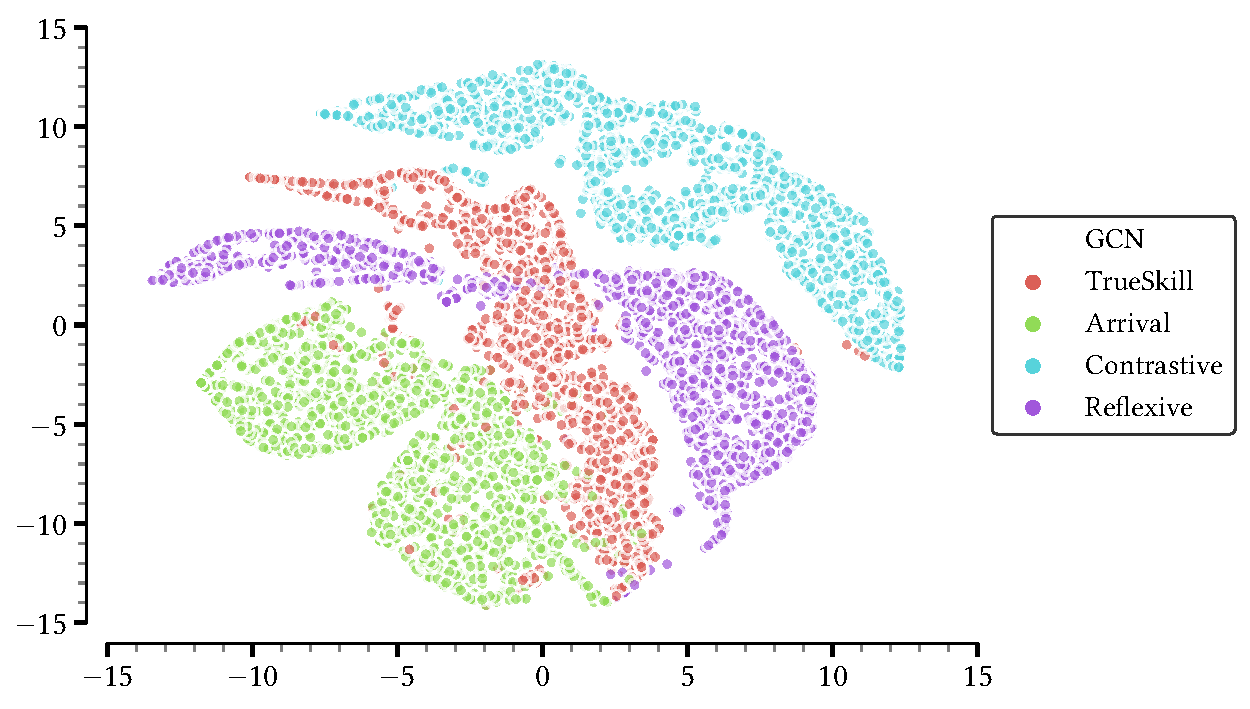
\includegraphics[scale=0.3]{figures/sne_plot.pdf}
  %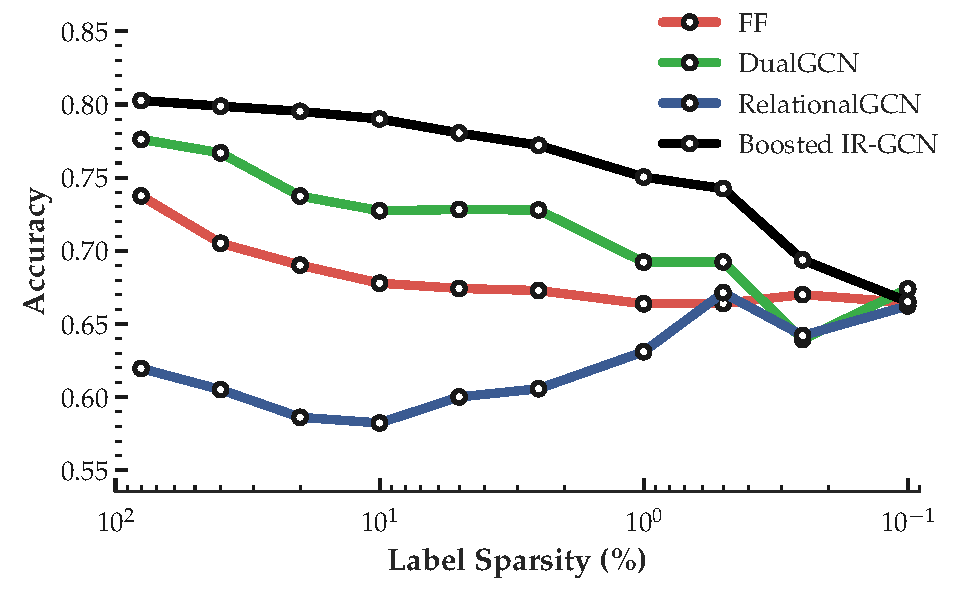
\includegraphics[height=4.2cm,width=0.85\linewidth]{figures/Label_Sparsity}
  %\vspace{-0.15in}
  \caption{\small \label{fig:sne} t-stochastic neighbor embedding (t-SNE) \cite{sne} distributions of the learned vertex representations by our model for Chemistry StackExchange. Each view learns a distinct vertex representation. Best viewed in color.}
  \vspace{-0.1in}
%\end{figure}
\end{wrapfigure}

Among individual views, Contrastive GCN performs best on all the communities. It even beats the best performing baseline DualGCN that uses all the relational views. Note that the contrastive view compares between the candidate answers to a question and uses our proposed contrastive modification to the convolution operation. Arrival Similarity follows Contrastive and then Reflexive. The superior performance of the Arrival Similarity view shows that early answers tend to get accepted and vice versa. It indicates that users primarily use CQA forums for quick answers to their queries. Also, recall that Reflexive predicts each vertex's label independent of other answers to the same question. Thus, the competitive performance of the Reflexive strategy indicates that vertex's features itself are well predictive of the label. TrueSkill Similarity performs at par or slightly worse than Reflexive. \Cref{fig:sne} presents t-SNE distributions \cite{sne} of the learned vertex representations ($\mathbf{Z}_i^K$) of our model applied to Chemistry StackExchange from Science category. Note that each view, including two views under Similarity by Contrast relation, learns a distinct vertex representation. Hence, all views are essential and contribute to our final performance.

Out of the baseline graph ensemble approaches, DualGCN performs significantly better than RelationalGCN by an average of around 26\% for all categories. Recall that in the RelationalGCN model, the convolution output of each view is linearly combined to compute the final output. Linear combination works well for knowledge graphs as each view can be thought of as a feature, and then it accumulates information from each feature. DualGCN is similar to our approach and trains different GCN for each view and later merges their results. However, it enforces similarity in vertex representations learned by each view. This restriction is not suitable for our induced-relationships as they are semantically different (contrastive captures contrast in features vs. similarity enforces label sharing).


%\section{Discussion}
%In this section, we first evaluate importance of each relational view for our boosted model. We then compare with approaches proposed to merge neural networks in general in other domains. Finally, we study robustness of our model to training label sparsity.

%\vspace{-0.1in}
\subsection{Ablation Study on Relation Types}
\begin{table}[h]
  \vspace{-0.0in}
  \small
  %\robustify\bfseries
  \begin{tabular}{l | S[round-mode=places,round-precision=2]@{\hspace{2mm}}|S[round-mode=places,round-precision=2]@{\hspace{2mm}}|S[round-mode=places,round-precision=2]@{\hspace{2mm}}| S[round-mode=places,round-precision=2]@{\hspace{2mm}}|S[round-mode=places,round-precision=2]}
  %\begin{tabular}{l | c | c| c| c|c}
    \toprule
  %  \textbf{Strategies} &
      % \textbf{SF} &
      % \textbf{ENG} &
      % \textbf{SCIFI} &
      % \textbf{PHYS}&
      % \textbf{WP}\\
       \textbf{\{ Relation Type\}} &
        \textbf{Tech} &
        \textbf{Culture} &
        \textbf{Life} &
        \textbf{Sci}&
        \textbf{Business}\\
      \midrule
      C & 71.23 &75.90 &78.71&72.99 & 76.85\\
    \{ TS, AS \} & 67.86 &74.15 &75.75&65.80& 76.13  \\
    R & 68.30 & 73.35 & 76.57 & 67.40 & 75.76 \\
    \{TS, AS \} + R & 69.28 & 75.50 &76.41 &70.11  &77.90 \\
    C + R & 73.04 & 77.66 & 80.25 &73.72 & 80.04 \\
    C + \{ TS, AS \} & 72.81 & 78.04 & 81.41 & 72.19 & 80.15\\
    C + \{ TS, AS \} + R & \bfseries 73.87 & \bfseries 78.74 & \bfseries 81.60&  \bfseries74.68&  \bfseries80.56 \\
    \bottomrule
  \end{tabular}
  \caption{\small \label{tab:relation} 5-fold Accuracy (in \%) comparison for different combination of relation types for our boosted model. Contrastive and Similarity by Contrast relations together performs similar to the final model.}
  \vspace{-0.15in}
\end{table}

We present the results of an ablation study with a different combination of relation types (Contrastive, Similarity, and Reflexive) used for the IR-GCN model in Table \ref{tab:relation}. We conducted this study on the biggest community from each of the five categories, i.e., ServerFault (Technology), English (Culture), Science Fiction (Life), Physics (Science), Workplace (Business).
Similarity by Contrast relation (TrueSkill and Arrival) used in isolation performs the worst among all the variants. Training Contrastive and Similarity by Contrast relation together in our boosted framework performs similar to our final model. Reflexive GCN contributes the least as it does not consider any neighbors.

\vspace{-0.1in}
\subsection{Aggregator Architecture Variants}
\label{sec:agg}
We compare our gradient boosting based aggregation approach with other popular methods used in literature to merge different neural networks discussed in \cref{item:aggregator}.

\begin{table}[h]
  \small
  %\robustify\bfseries
  \vspace{-0.15in}
  \begin{tabular}{l | c | c| c| c|c}
    \toprule
    % \textbf{Method} &
    %   \textbf{SF} &
    %   \textbf{ENG} &
    %   \textbf{SCIFI} &
    %   \textbf{PHYS}&
    %   \textbf{WP}\\
    \textbf{Method} &
     \textbf{Tech} &
     \textbf{Culture} &
     \textbf{Life} &
     \textbf{Sci}&
     \textbf{Business}\\
      \midrule
    Stacking~\cite{Stacking} &68.58 & 74.44 & 79.19 & 70.29 &75.50  \\
    Fusion~\cite{Fusion18}  &72.30 &77.25 & 80.79 & 73.91 &79.01 \\
    NeighborAgg~\cite{graphsage,relationalGCN}  &69.29 &74.28 & 77.94 & 68.42 &78.64   \\
    IR-GCN & \bfseries 73.87 & \bfseries 78.74 & \bfseries 81.60&  \bfseries74.78&  \bfseries80.56 \\
    \bottomrule
  \end{tabular}
  \caption{\small \label{tab:agg} 5-fold Accuracy (in \%) comparison of different aggregator architectures. These architectures perform worse than Contrastive GCN. Fusion performs similarly but is computationally expensive.}
  \vspace{-0.2in}
\end{table}

Table \ref{tab:agg} reports the accuracy results for these aggregator variants as compared to our model. Our method outperforms all the variants with Fusion performing the best. This worse performance reaffirms that existing aggregation models are not suitable for our problem. Note that these approaches perform worse than even Contrastive GCN except Fusion. The fusion approach performs similarly to our approach but is computationally expensive as the input size for each IR-GCN in fusion is linear in the number of all views in the model.

\subsection{Textual Features}
Most of the current literature focuses on using textual features for Answer Selection. In this section, we compare our proposed IR-GCN model to a popular text-based model~\cite{Tan2015}. %proposed for answer selection.

\noindent
\textbf{QA-LSTM/CNN \cite{Tan2015}} uses a stacked bidirectional LSTM model followed by convolution filters to learn embeddings for the question and answer text separately. They then rank answers in decreasing order of the cosine similarity between question and answer embeddings.

  %\item{\textbf{biLSTM+CNN} The basic biLSTM model was extended to learn more composite embedding by using convolution filters on biLSTM output.}
\noindent
\textbf{Textual Similarity (T-GCN)} We create a \textit{Similarity by Contrast} view that connects answers authored by a user where her answer's text is significantly similar (dissimilar) to the question's text than the other competing answers. We used cosine similarity on the learned question and answer embeddings from the QA-LSTM approach as the similarity function.

\noindent
\textbf{IR-GCN + T-GCN} extends our proposed model to also include the Textual Similarity as the third \textit{Similarity by Contrast} view in addition to Arrival and TrueSkill views.
\begin{table}[h]
  \small
  %\robustify\bfseries
  \centering
    \vspace{-0.0in}
  \begin{tabular}{l | S[round-mode=places,round-precision=2]S[round-mode=places,round-precision=2]S[round-mode=places,round-precision=2]S[round-mode=places,round-precision=2]S[round-mode=places,round-precision=2]}
    \toprule
    \textbf{Method} &
      \textbf{Tech} &
      \textbf{Culture} &
      \textbf{Life} &
      \textbf{Sci} &
      \textbf{Business}\\
      \midrule
    QA-LSTM/CNN\cite{Tan2015} & 66.49 & 71.70 & 69.42 & 62.91 & 72.55 \\
    FF~\cite{JendersKN16} & 68.30 & 73.35 & 76.57 & 67.40 & 75.76 \\
    T-GCN & 69.25 & 73.77 & 76.39 & 67.79 & 77.08\\
    IR-GCN & 73.87 & 78.74 & 81.60 & 74.68 & 80.56 \\
    IR-GCN + T-GCN & 73.89 & 78.00  & 81.07 & 74.49 & 78.86\\
    \bottomrule
  \end{tabular}
  \caption{\small \label{tab:text} 5-fold Accuracy comparison of text-based baseline and textual similarity GCN with IR-GCN.}
    \vspace{-0.2in}
\end{table}

In general, the text-based baseline, QA-LSTM, performs worse than even reflexive GCN, as shown in Table \ref{tab:text}. Note that reflexive GCN employs a feedforward model on the activity and user features used in our experiments. This is a surprising result as most of the current literature focus on textual features for the task. Our results indicate that non-textual features are useful too for the answer selection task on StackExchange communities.

Textual Similarity GCN performs better than QA-LSTM and Reflexive GCN. Even though we use the output of QA-LSTM to construct the graph for T-GCN, the graph improves performance as it connects answers across different questions. However, adding the T-GCN view in our proposed IR-GCN model decreases the performance slightly. One possible explanation could be that similarity by contrast views based on user features (Arrival similarity and TrueSkill similarity) are not compatible with views based on textual features.

% \begin{table}[h]
%   \small
%   %\robustify\bfseries
%   \centering
%   \begin{tabular}{l | S[round-mode=places,round-precision=2]S[round-mode=places,round-precision=2]S[round-mode=places,round-precision=2]S[round-mode=places,round-precision=2]S[round-mode=places,round-precision=2]}
%     \toprule
%     \textbf{Method} &
%       \textbf{Tech} &
%       \textbf{Culture} &
%       \textbf{Life} &
%       \textbf{Sci} &
%       \textbf{Business}\\
%       \midrule
%     QA-LSTM/CNN\cite{Tan2015} & 66.49 &  & 69.42 & 62.91 & 72.55 \\
%     FF~\cite{JendersKN16} & 66.00 & 72.22 & 69.85 & 63.63 & 75.57 \\
%     CS-GCN & 66.06 & 72.35 & 71.88 & 64.14 & 75.69 \\
%     IR-GCN & 66.56 & 72.92 & 72.54 & 65.11 & 75.95 \\
%     IR-GCN + CS-GCN & 66.49 & 73.17 & 72.85 & 65.29 & 75.86 \\
%     \bottomrule
%   \end{tabular}
%   \caption{\small \label{tab:textfeature} 5-fold Accuracy comparison of content-based baseline and content-similarity GCN with learnt content embeddings as features in the GCN.}
% \end{table}
%
% We further replaced our activity based features with the learned embeddings obtained after training the QA-LSTM/CNN~\cite{Tan2015} model. We observed that performance of all approaches went down slightly when using content features (Table \ref{tab:textfeature}). As we noted before, GCNs aggregate features among the neighbors. In our similar contrast view, it is not favorable to aggregate content features among the neighbors as we connect answers catering to different questions. Thus, aggregating content features will create noise in the dataset.

\vspace{-0.2in}
\subsection{Discriminative Magnification effect}

% \begin{figure}[tbh]
%   \centering
%   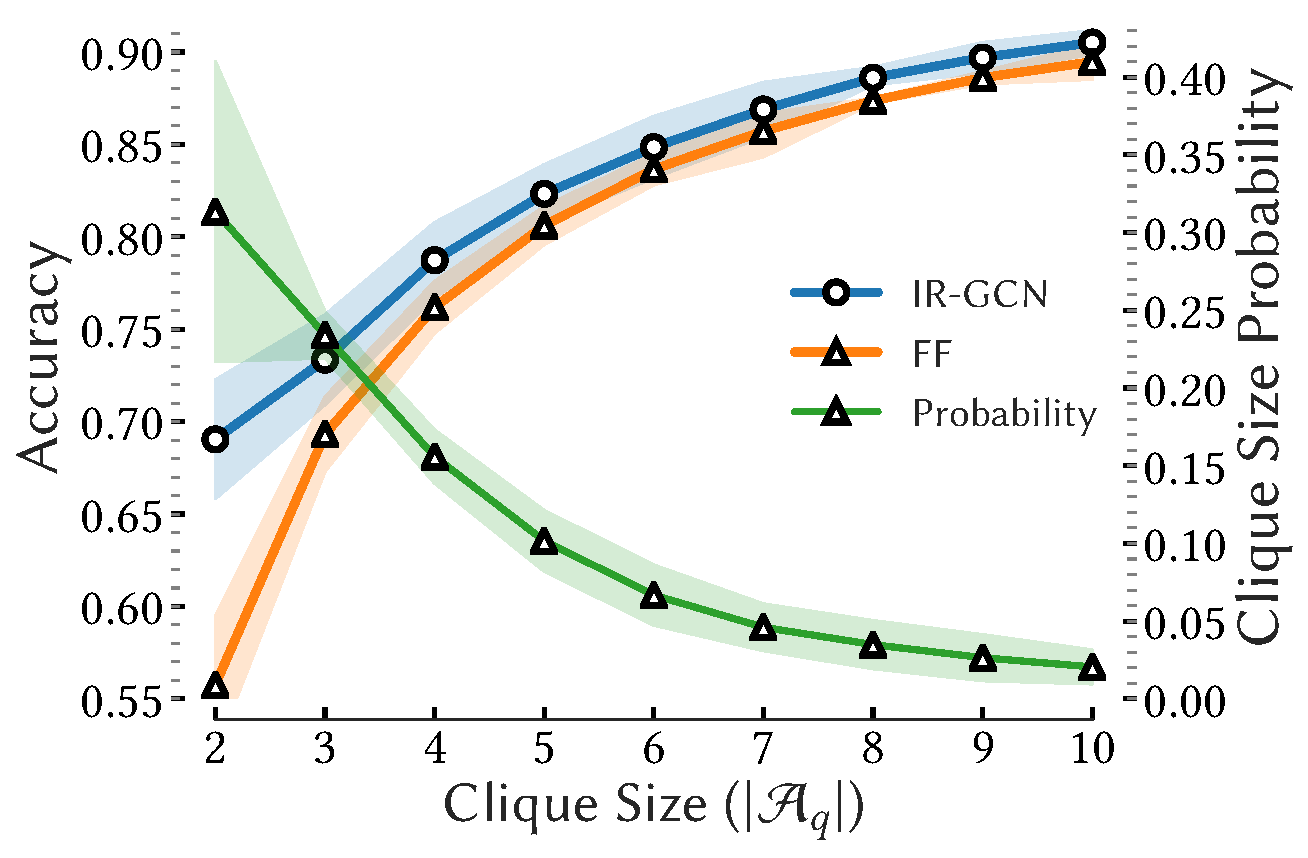
\includegraphics[scale=0.3]{figures/clique_acc.pdf}
%   %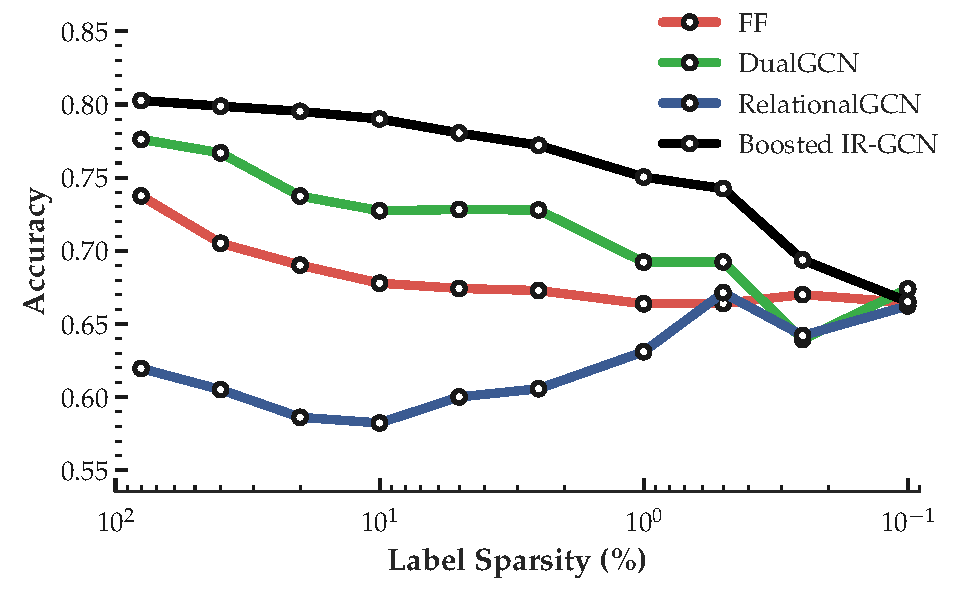
\includegraphics[height=4.2cm,width=0.85\linewidth]{figures/Label_Sparsity}
%   \vspace{-0.12in}
%   \caption{\small \label{fig:clique} Accuracy of our IR-GCN model compared to the FF model with varying clique size (i.e. number of answers to a question, $\vert \mathcal{A}_q \vert$) for Contrastive view . %The results are reported for the largest StackExchange community in all five categories.
% We report averaged results over the largest community of all categories. Our model performs much better for smaller cliques, and the effect diminishes for larger cliques (\cref{eq:contrast}). 80\% of the questions have $< 4$ answers.}
%   \vspace{-0.15in}
% \end{figure}

We show that due to our proposed modification to the convolution operation for contrastive view, we achieve \emph{Discriminative Magnification effect} (\cref{eq:contrast}). Note that the difference is scaled by Clique size ($1 + 1/n-1$), i.e. number of answers to a question, $\vert \mathcal{A}_q \vert$. Figure \ref{fig:clique} shows the accuracy of our IR-GCN model as compared to the FeedForward model with varying clique size. Recall that the FeedForward model predict node labels independent of other nodes and is not affected by clique size. We report average results over the same five communities as above. We can observe that increase in accuracy is much more for lower clique sizes (13\% improvement for $\vert \mathcal{A}_q \vert = 2$ and 4\% for $\vert \mathcal{A}_q \vert = 3$ on average). The results are almost similar for larger clique sizes. In other words, our model significantly outperforms the FeedForward model for questions with fewer candidate answers. However, around 80\% of the questions have very few answers($< 4$), and thus this gain over FF is significant.

\vspace{-0.2in}
\subsection{Label Sparsity}

\begin{figure}[tbh]
  \begin{subfigure}{0.4\textwidth}
    \centering
    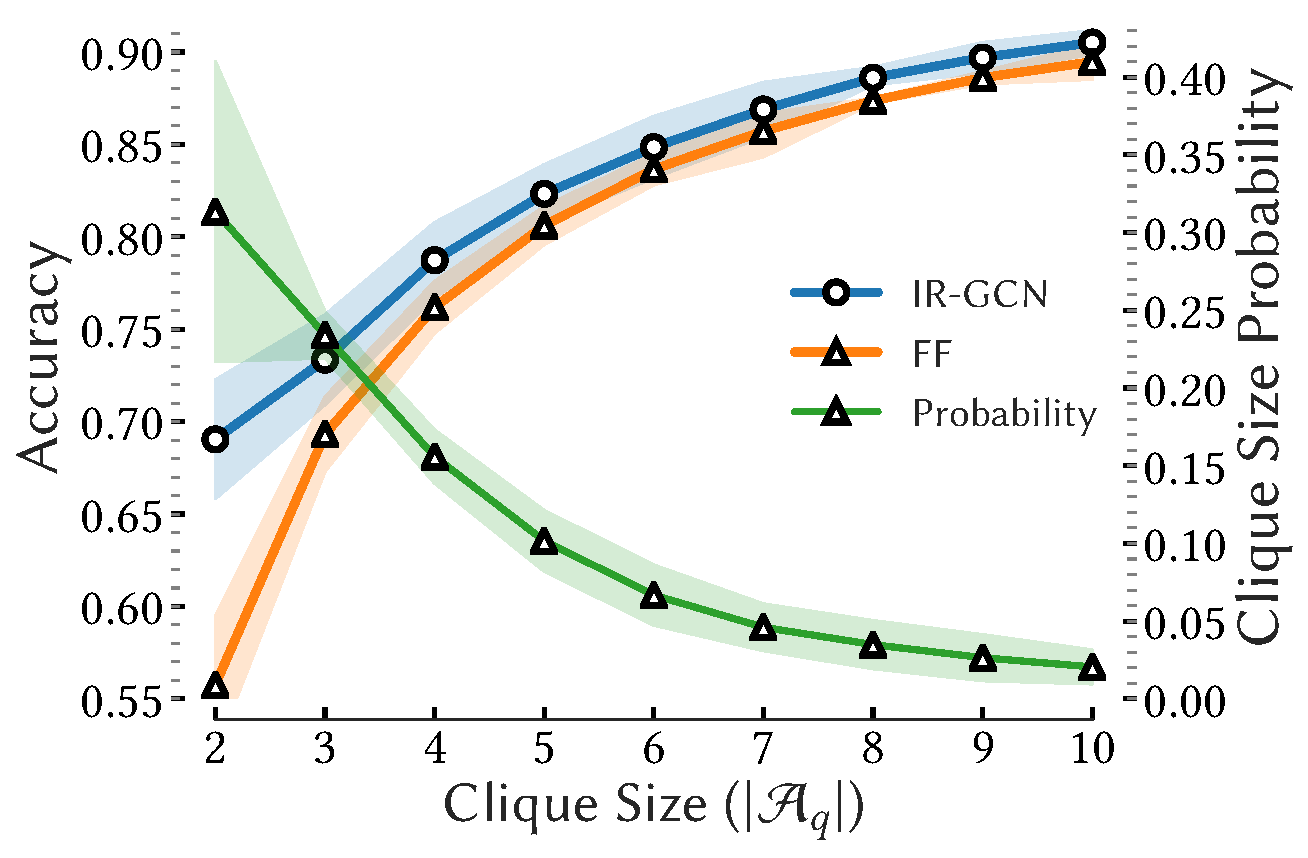
\includegraphics[scale=0.26]{figures/clique_acc.pdf}
    %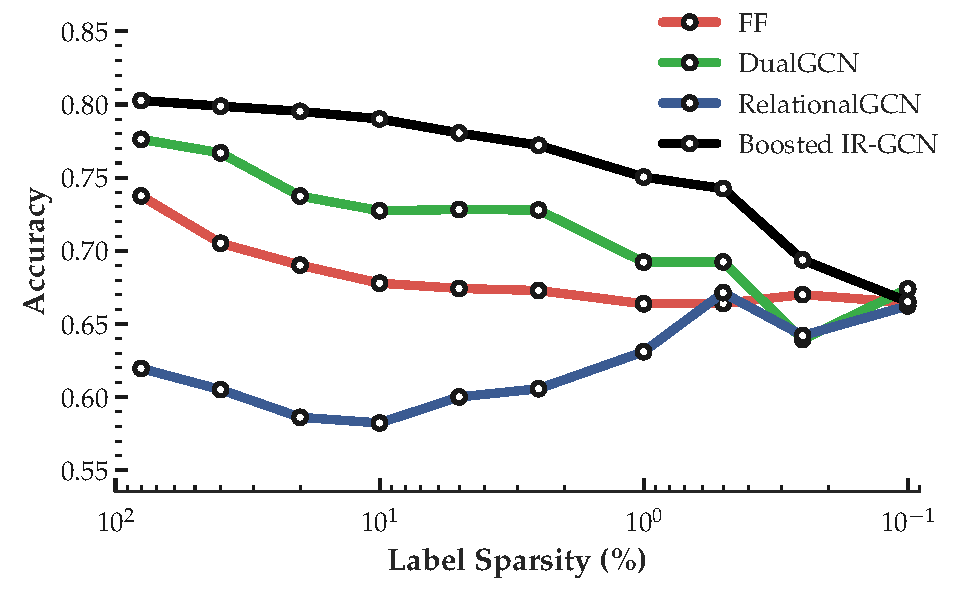
\includegraphics[height=4.2cm,width=0.85\linewidth]{figures/Label_Sparsity}
    \caption{\small \label{fig:clique}}
    %\vspace{-0.12in}
  \end{subfigure} \hspace{0.3in}
  \begin{subfigure}{0.55\textwidth}
      \centering
  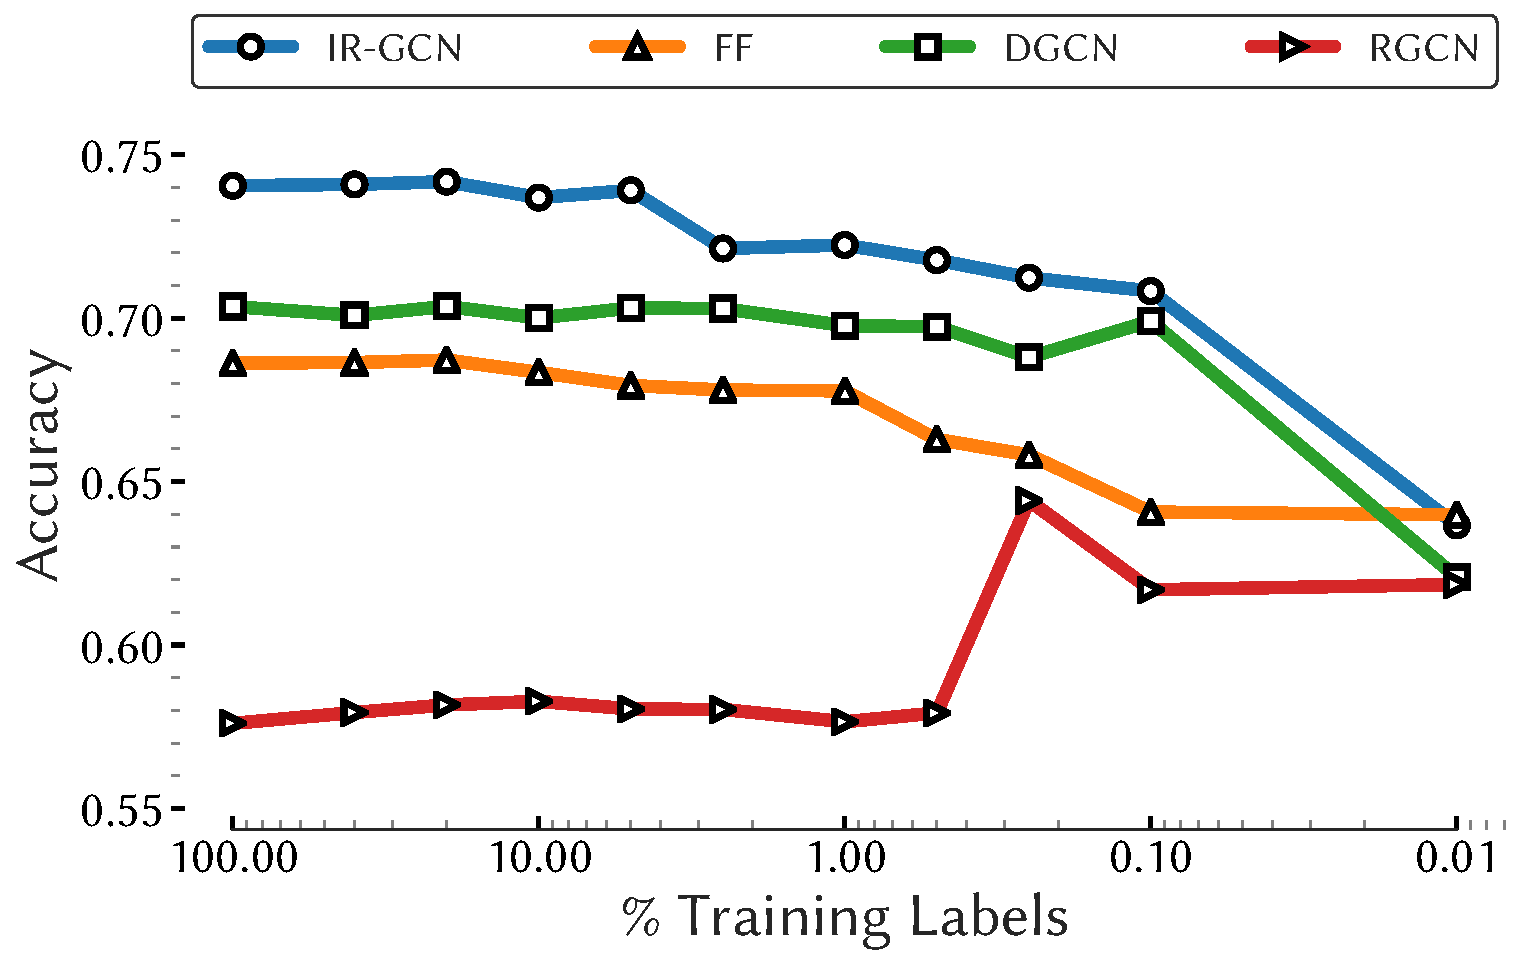
\includegraphics[scale=0.25]{figures/sparsity_acc_physics.pdf}
  %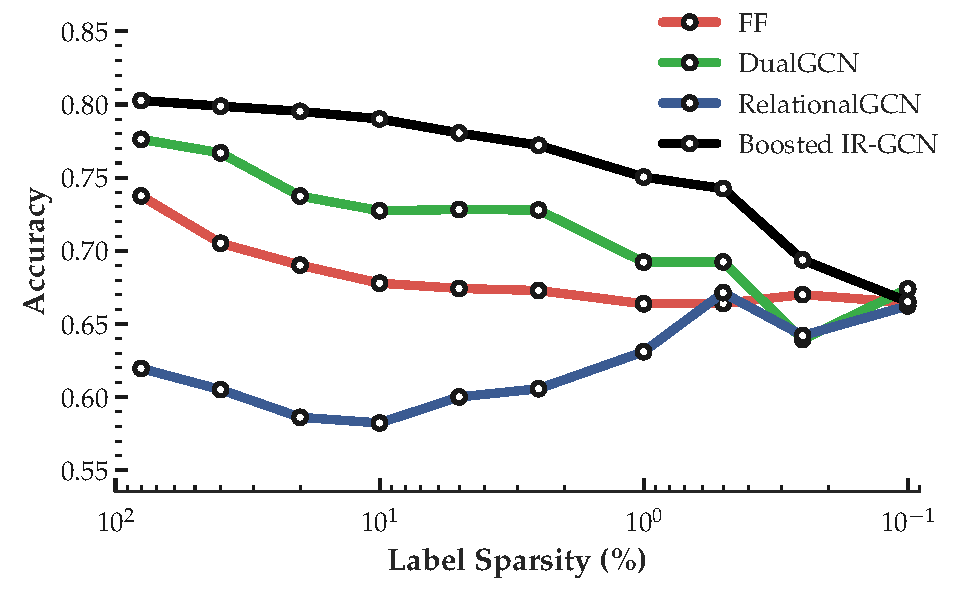
\includegraphics[height=4.2cm,width=0.85\linewidth]{figures/Label_Sparsity}
  %\vspace{-0.2in}
  \caption{\small\label{fig:labelsparsity} }
  \end{subfigure}
  %\vspace{-0.2in}
  \caption{\small a) Accuracy of our IR-GCN model compared to the FF model with varying clique size (i.e., number of answers to a question, $\vert \mathcal{A}_q \vert$) for Contrastive view. %The results are reported for the largest StackExchange community in all five categories.
We report averaged results over the largest community of all categories. Our model performs much better for smaller cliques, and the effect diminishes for larger cliques (\cref{eq:contrast}). 80\% of the questions have $< 4$ answers. \\
b) Change in accuracy with varying training label rates for Physics StackExchange. Our model is more robust to label sparsity than other relation ensemble approaches. RGCN works better with fewer labels as contrastive relation introduces noise in the model. At extreme sparsity, all approaches converge to the same value indicating random selection.
}
\end{figure}
Graph Convolution Networks are robust to label sparsity as they exploit graph structure and are thus heavily used for semi-supervised settings. Figure \ref{fig:labelsparsity} shows the change in accuracy for Physics StackExchange from the Science category at different training label rates. Even though our graph contains disconnected cliques, IR-GCN still preserves robustness to label sparsity.
In contrast, the accuracy of the FeedForward model declines sharply with less label information. Performance of DualGCN remains relatively stable while Relational GCN's performance increases with a decrease in label rate. Relational GCN assumes each view to be of similarity relation, and thus, adding contrastive relation introduces noise in the model. However, as the training labels become extremely sparse, the training noise decreases that leads to a marked improvement in the model. In the case of a meager label rate of 0.01\%, all approaches converge to the same value, which is the expectation of theoretically random selection. We obtained similar results for the other four StackExchange communities but omitted them for brevity.

% \subsection{Change in Accuracy with Clique Size}

\begin{comment}
\subsection{Contrastive GCN Analysis}
\label{ref:analysis}
The ability of neural networks to perform classification in sparse high-dimensional manifolds has been studied in past work, especially in the context of adversarial learning \cite{lu2017safetynet}. We employ the ReLU activation function in our convolution layers and study the outputs of the $k$th layer, i.e. embeddings with k-order locality. This transformation breaks the input space into cells with smooth gradients within each cell, at whose boundaries the piecewise linear function changes (i.e. the likelihood of the two classes of answers).

% In the context of adversarial learning \cite{safetynet} propose the existence of p-domains or cells in the learned manifold, representing a piecewise linear mapping of the transformed features to the class labels. The generalization neutrality property is particularly interesting. Both train and test samples are highly unlikely to lie in p-domains since the number of examples is much smaller than the capacity of the neural network to fit these regions. Weight decay can incentivize relatively small changes in the gradient across these regions resulting in smoother changes.  the ability of the network to fit such regions in the data manifold?

We ask a specific question in the context of our Contrastive IR-GCN. \emph{What is the impact of the layerwise discriminative magnification induced by our formulation?} Discriminative magnifications results in improved separability of the two classes in the later convolving layers, an effect we earlier demonstrated with a sample network in \cref{fig:contrast}. This positively impacts the ability of the model to explain the observed data points (i.e create p-domains that are well aligned with the contrastive samples provided) and improve the generalizability of the learned model to unseen data points. However, it is important to maintain sufficient regularization with weight decay to prevent sparse regions exhibiting sharp gradients which could affect model performance.

The capacity of our model can also be quantified in terms of the VC dimension of the aggregated classifier against the individual learners. Gradient boosting with multiple relation learners (each of which captures a specific aspect of node locality via graph convolution on the induced relations) could boost the capacity of the joint model, enabling better generalization and a more accurate fit in the data manifold (i.e. higher capacity to fit regions to fine distinctions).

Let us denote the upper bound of the VC dimension or capacity of each individual learner as D (If the individual learners do not have identical capacity, the minimum can be used to compute a lower bound on the aggregated learner capacity). Then the gradient boosted learner with T classifiers has a bound on it's capacity~\cite{shalev2014understanding} given by,
\begin{equation*}
\mathcal{VC}_{Agg}  = T \times (D+1) \times(3 \log(T.(D+1))+2)
\label{vcdim}
\vspace{-0.03in}
\end{equation*}

Thus we identify two potential reasons for our performance gains, first the discriminative magnification effect which also supports the strong individual performance of the contrast view, and second the gain in capacity from boosting, which could explain it's advantage over competing aggregation methods.

\end{comment}


\vspace{-0.2in}
\subsection{Limitations} We do recognize certain limitations of our work. First, %we do not deal with content in our model. Our focus in this work is to exploit structural properties between tuples. We believe that adding content will further improve our results. Second, 
we focus on equivalence relations that induce a graph comprising cliques. While cliques are useful graph objects for answer selection, equivalence relations may be too restrictive for other problems (e.g., the relation is not transitive). However, our modular framework does apply to arbitrary graphs, except that~\Cref{eq:restrictk} will no longer be an \emph{exact} convolution but be an approximation. Second, we assume no evolution in author skills. This assumption is not true as users evolve with experience. We aim to address this in future work.



%First, creating induced links require domain knowledge or empirical analysis of the dataset. Second, we do not exploit the content in our model. Although we achieve significant improvements with a basic feature set, the content could be helpful in semi-supervised settings. Third, we assume no evolution in author skills. This assumption is not true as users evolve with experience. We aim to address this in future work.
%\vspace{5pt}




%Our model showed significant gains over state-of-the-art baselines for combining information from semantically different relational links in a graph. Our model is also more robust to training label sparsity as compared to other aggregator GCN approaches. We reasoned that the performance gains achieved by our aggregation strategy can be attributed in part to the enhanced learning capacity of the boosted model and the effect of discriminative feature magnification. Finally, we presented a few limitations and possible future extensions.




%\textbf{Observation 1} - Inducing p-domains in the learned manifold to separate classes\\\\
%In this explanation, we assume the graph convolutional network uses ReLU and weight decay because they are representative, make it easier to explain, and likely to extend to other conditions with some modifications. We have a network with N layers of ReLU's and study the values at the output of the $k$th layer of ReLUs (k-order locality). This is a piecewise linear function of x. Such functions break up the input space into cells, at whose boundaries the piecewise linear function changes (i.e., the likelihood of the two classes of answers). Now assume that for some class y (+ or -1) there exist p-domains (union of cells) D in the input space such that: (a) there are no or few examples in the p-domain; (b) the measure of D under P(X) is small; (c) The probability of a specific class (either + or -1) is large inside D and small outside D. We will use the term "p-domain" to refer to domains with these properties, inspired by past work \cite{safetynet}. The notion of p-domains has been used to study the discontinuities introduced by neural network based classifiers in high dimensional spaces \cite{safetynet}.
%
%
%\textbf{How does discriminative magnification impact the p-domains induced by the graph convolutional learner?\\}
%Generalization-neutral: The requirement that p-domains have small measure in P(X) means that both train and test examples are highly unlikely to lie in p-domains (given the high dimensionality of the induced space as well as the relatively small number of training samples). A system with p-domains could thus generalize well to new unseen examples. Note that the discriminative magnification effect achieved in subsequent convolutional layers positively impacts the ability of the model to explain the observed data points (i.e create p-domains that are well aligned with the contrastive samples provided). This in turn is likely to improve the generalizability of the learned model to unseen data points, and could hence explain the strong performance observed with the contrast learner.
%
%
%\textbf{Observation 2} - Gradient boosting can further amplify the ability of neural networks to exploit discriminative magnification \\\\
%$$Add VC dimension equation here$$
%\end{comment}
